
\chapter{Week 7 -- SOC Estimation, part 1}

\section{Abstract}
This report presents an implementation of several basic algorithms used for state-of-charge estimation. Using noisy input-output data from a simulation of a 2RC equivalent circuit model,
three methods of SoC determination -- namely the Coulomb counting, lookup using filtered terminal voltage and the combination of both -- were implemented and validated against reference data. All algorithms are executed for various values of hyperparameters to assess their robustness and errors caused by gradual drift or deviation in initial conditions. The accuracy of estimation is measured using the root-mean-square error.

\section{Cell model}

The chosen battery model considers only the dynamics of the $SoC$ and otherwise represents the cell as a static system
\begin{equation}
    \begin{split}
        \dot{SoC} &= -\frac{1}{C} i, \\
        \Ubat &= \OCV(SoC) - i R_0(SoC),
    \end{split}
    \label{eq:7-cont}
\end{equation}
with nonlinear output equation, where the system input $i$ denotes the flowing current, state $SoC \in \left[0, 1\right]$ is the state of charge, $\Ubat$ is the battery terminal voltage (system output) and the total capacity $C$, open circuit voltage $\OCV(SoC)$ and internal resistance $R_0(SoC)$ are (possibly $SoC$-dependent) model parameters. Numeric values of all model parameters are provided as a part of the assignment. Forward Euler discretization of \eqref{eq:7-cont} with sampling period $T_s = \SI{0.1}{\second}$ yields a simple system
\begin{equation}
    \begin{split}
        SoC(k+1) &= SoC(k) - \alpha \frac{T_s}{C} i(k), \\
        \Ubat(k) &= \OCV(SoC(k)) - i(k) R_0(SoC(k)),
    \end{split}
    \label{eq:7-disc}
\end{equation}
appropriate for the implementation in code. The state equation was extended with a scaling factor $\alpha$ that handles the conversion of capacity $C$ from ampere-hours to coulombs and the transformation of $SoC$ from $\left[0, 1\right]$ to percentage.

\begin{figure}
    \centering
    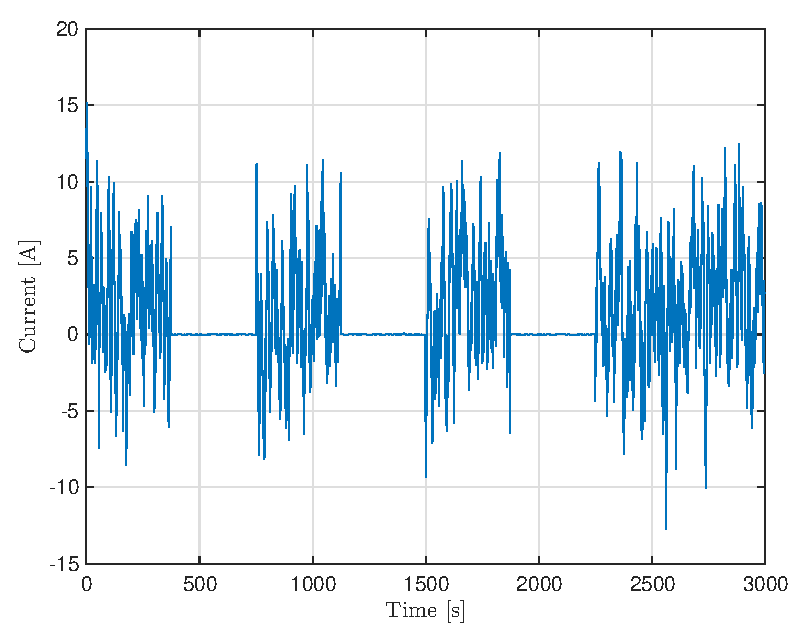
\includegraphics[width=0.5\textwidth]{figures/7/validation-I.eps}
    \caption{Current waveform used during all simulations.}
    \label{fig:7-validation-I}
\end{figure}

\section{Algorithm implementation}

The implementation was verified by simulating the model using provided parameter values and several sets of initial conditions and comparing them against waveforms obtained during the reference experiment. As shown in Fig. \ref{fig:7-validation-I}, the reference current represents a highly dynamic profile that combines high charging and discharging currents interleaved by several minutes-long rest periods with no current flow. This waveform is appropriate for demonstrating various SoC estimation algorithms as it excites both long-term and short-term cell dynamics.



\begin{figure}
    \centering
    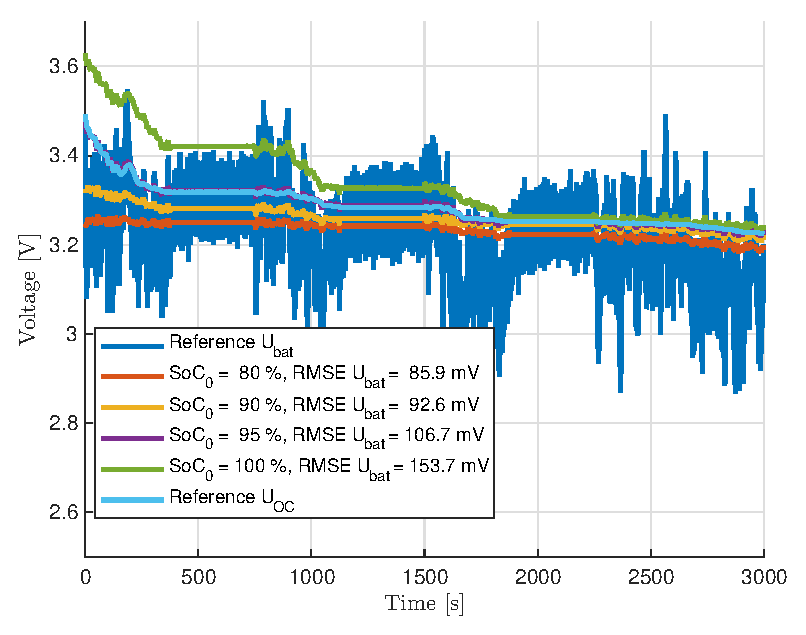
\includegraphics[width=0.5\textwidth]{figures/7/validation-Ubat.eps}
    \caption{Comparison of battery terminal voltages during simulation and the reference experiment.}
    \label{fig:7-validation-Ubat}
\end{figure}

Since the model \eqref{eq:7-disc} is very simple, large discrepancies between the reference waveform and simulation outputs are expected, as shown in Fig. \ref{fig:7-validation-Ubat}. Simulated terminal voltages differ by more than 80 mV using the RMSE metric, as they do not follow relatively fast dynamics observable in the reference waveform. The reason becomes apparent on closer inspection -- reference waveforms were generated using the 2RC equivalent circuit model, whereas the simulation only uses $R_0$ (neglecting $R_1$ and $R_2$). Neglecting the voltage drop across these resistances results in a far lower magnitude of voltage ripple in response to dynamically varying current.

\subsection{Coulomb counting}
\label{sec:7-cc}

The aforementioned systematic error is not a major issue for simple estimation of $SoC$, which, in the simple case without state observers, is completely unaffected by incorrect model impedance.The \textit{Coulomb counting} algorithm evaluates the state equation in \eqref{eq:7-disc}, performing an inherently open-loop integration of the flowing current. This way $SoC$ can be calculated without any knowledge about $\Ubat$, making this method useful when only a low-fidelity model is available.

\begin{figure}[bp]
    \centering
    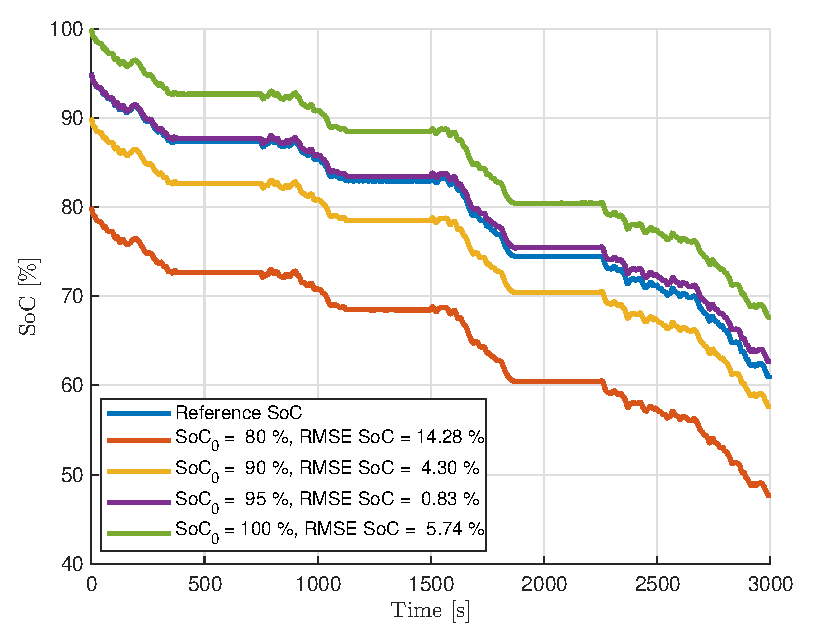
\includegraphics[width=0.5\textwidth]{figures/7/validation-SOC.eps}
    \caption{Comparison of simulated SoCs with the reference experiment.}
    \label{fig:7-validation-SOC}
\end{figure}

This is illustrated in Fig. \ref{fig:7-validation-SOC} -- since the $SoC$ evolution only depends on the accuracy of current measurement $i$ and cell capacity $C$ (and the coulombic efficiency $\eta$ when not neglected), estimates of $SoC$ for various initial conditions evolve "in parallel" and the error neither shrinks nor grows over time. However, even when the algorithm is initialized very close to the true initial state of charge (roughly 95 \%), it tends to drift away over time. Open-loop integration accumulates errors and has no means of self-correction.







\begin{figure}[tbp]
    \centering

\begin{subfigure}{0.49\textwidth}
    \centering
    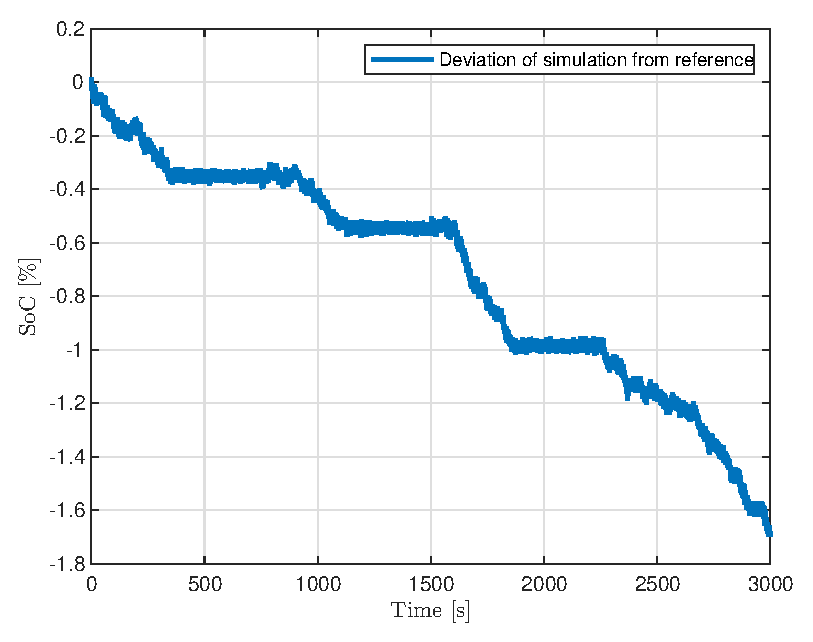
\includegraphics[width=\textwidth]{figures/7/validation-deviation-in-time.eps}
    \caption{Plotted over time.}
    \label{fig:7-validation-deviation-in-time}
    \end{subfigure}
    \hfill
    \begin{subfigure}{0.49\textwidth}
    \centering
    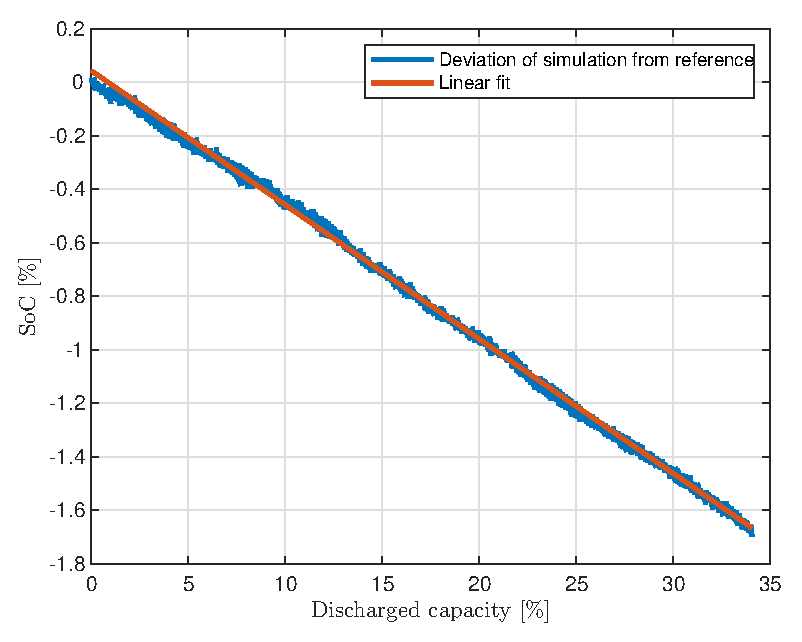
\includegraphics[width=\textwidth]{figures/7/validation-deviation.eps}
    \caption{Plotted w.r.t the Depth of Discharge (DoD).}
    \label{fig:7-validation-deviation}
    \end{subfigure}
    
    \caption{Gradual deviation of the reference and simulated SoC.}
    \label{fig:7-deviation}
\end{figure}

This behaviour can be observed in detail on Fig. \ref{fig:7-deviation}. Several possible factors may cause the simulated waveform to drift away from the reference $SoC$ over the course of the experiment, as shown in Fig. \ref{fig:7-validation-deviation-in-time}. Some insight into probable causes of the drift can be gained by looking at Fig. \ref{fig:7-validation-deviation}, where the error is plotted against the percentage of capacity discharged. Observing the highly linear dependence (linear fit achieves RMSE only 0.016 \% $SoC$), one can conclude that the error is purely multiplicative and hence could be fixed by recalibrating the current sensor, recalculating the cell capacity $C$ or possibly by extending the model with coulombic efficiency $\eta$, as the simulated output tends to overestimate the amount of charge remaining in the battery.

\subsection{Open circuit voltage lookup}
\label{sec:7-ocv}

\begin{figure}[b]
\centering
\begin{minipage}{0.49\textwidth}
    \centering
    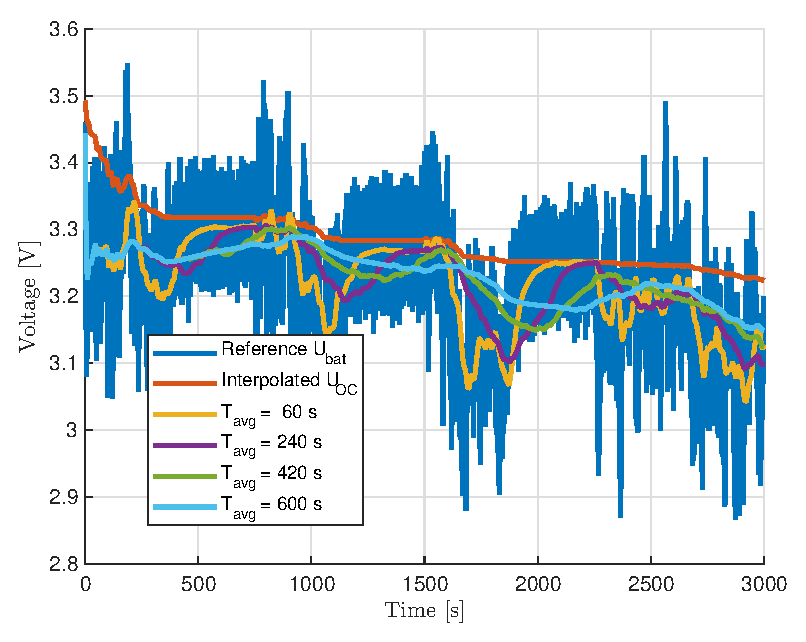
\includegraphics[width=\textwidth]{figures/7/OCV-Ubat.eps}
    \caption{$\OCV$ estimates for various values of $T_\text{avg}$.}
    \label{fig:7-OCV-Ubat}
\end{minipage}
\hfill
\begin{minipage}{0.49\textwidth}
    \centering
    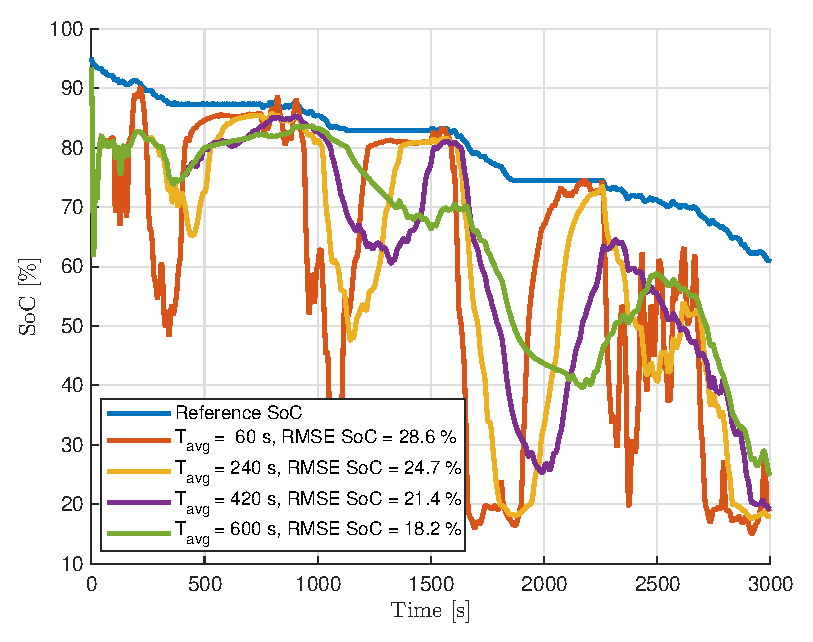
\includegraphics[width=\textwidth]{figures/7/OCV-SOC.eps}
    \caption{SoC estimates for various values of $T_\text{avg}$.}
    \label{fig:7-OCV-SOC}
\end{minipage}

\end{figure}

In contrast to Coulomb counting utilizing the measurement of battery current only, an alternative method uses only the measurement of battery terminal voltage $\Ubat$. Calculating a moving average of length $\Tavg$ over the recorded $\Ubat$ yields an approximation of the $\OCV$ that is subsequently used as an argument for table lookup.
Fig. \ref{fig:7-OCV-Ubat} shows how well the algorithm approximates the actual $\OCV$ with various setting of the hyperparameter $\Tavg$. A clear trend manifests, i.e. when $\Tavg$ is shorter, the algorithm is incapable of rejecting fast voltage drops when the cell is loaded, but it recovers quite quickly during the resting period. On the other hand, using a long averaging period $\Tavg$ results in stable $\OCV$ estimates (dynamically varying current goes through heavier filtering), but the approximation never approaches the actual $\OCV$ since averaging is longer than the resting period.

The same conclusion can be made when looking at Fig. \ref{fig:7-OCV-SOC} presenting $SoC$ estimates for various values of the hyperparameter $\Tavg$. Shorter $\Tavg$ yields an estimate with a larger variance that recovers quickly once the cell is allowed to rest. Longer $\Tavg$ ensures proper filtration of the estimate but simultaneously causes the estimate's mean value to deviate from the actual $SoC$. In this case, the algorithm underestimates the actual $SoC$ since the reference waveform reaches higher discharge currents than charging currents; therefore, the mean of $\Ubat$ is lower than $\OCV$.





\subsection{Coulomb counting with reset}
\label{sec:7-ccr}

Advantages of both previously analyzed algorithms can be merged to achieve the great stability of Coulomb counting and the robustness to incorrect initial conditions characteristic to the $\OCV$ lookup. The combined algorithm, from now on denoted as \textit{Coulomb counting with reset}, integrates the flowing current just like normal Coulomb counting. But whenever a resting period longer than $\Tdelay$ is detected, the measured terminal voltage $\Ubat$ is used as $\OCV$ to correct the $SoC$ estimate, removing any accumulated error.

\begin{figure}[htbp]
    \centering

\begin{subfigure}{0.49\textwidth}
    \centering
    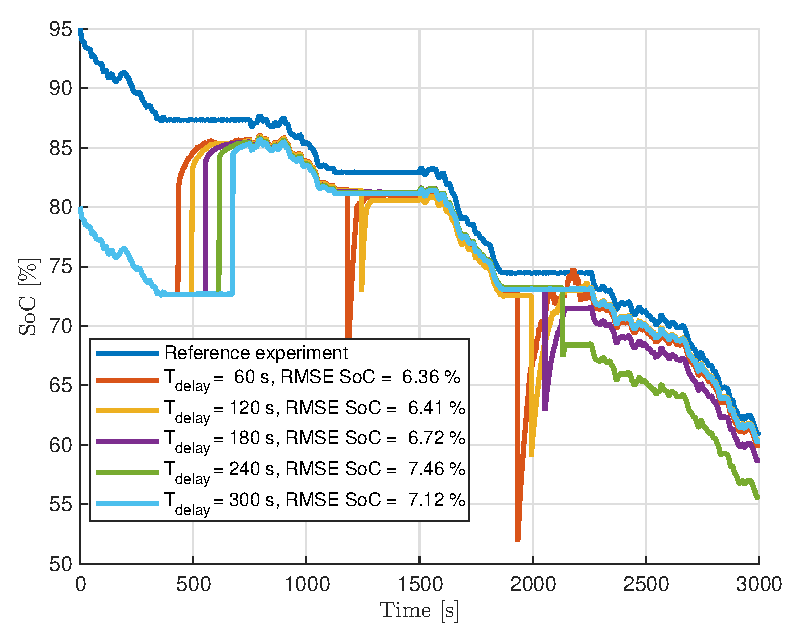
\includegraphics[width=\textwidth]{figures/7/combination-SOC.eps}
    \caption{SoC estimates for various hyperparameter values $T_\text{avg}$.}
    \label{fig:7-combination-SOC-macro}
    \end{subfigure}
    \hfill
    \begin{subfigure}{0.49\textwidth}
    \centering
    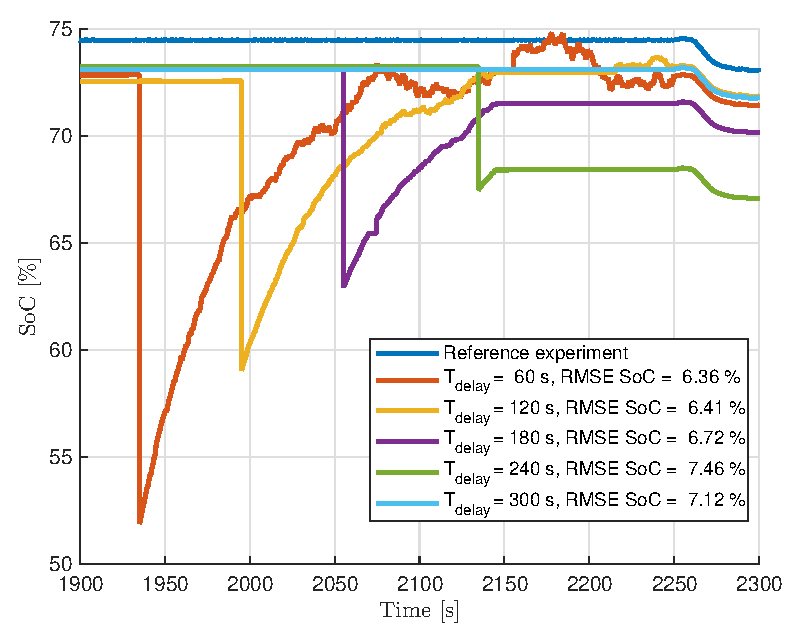
\includegraphics[width=\textwidth]{figures/7/combination-SOC-detail.eps}
    \caption{Detailed demonstration of reset behavior for various $T_\text{avg}$.}
    \label{fig:7-combination-SOC-detail}
    \end{subfigure}
    
    \caption{Demonstration of the \textit{Coulomb counting with reset} algorithm.}
    \label{fig:7-combination-SOC}
\end{figure}

This method has a hyperparameter $\Tdelay$, whose influence is illustrated in Fig. \ref{fig:7-combination-SOC}. When the current flow is interrupted at $t \approx \SI{380}{\second}$ and the cell is allowed to rest, $\Tdelay$ in some sense determines the amount of time given to the terminal voltage $\Ubat$ to converge to $\OCV$. After this delay elapses, the algorithm assumes that the $\Ubat$ has settled and uses its value to reset the integration.
The general trend regarding $\Tdelay$ can be inferred from Fig. \ref{fig:7-combination-SOC-detail} -- when the value gets larger,
the $SoC$ estimate is smoother (more filtered and less prone to short-term random walks), but extending $\Tdelay$ to infinity is not useful, as once it becomes longer than any reasonable resting period, the algorithm degenerates back to pure Coulomb counting without resets.
On the other hand, shorter $\Tdelay$ results in more frequent resets of the coulomb counting algorithm that occur even when $\Ubat$ is not fully settled, causing unwanted downwards spikes visible across the whole experiment in Fig. \ref{fig:7-combination-SOC-macro}.


\begin{figure}
    \centering
    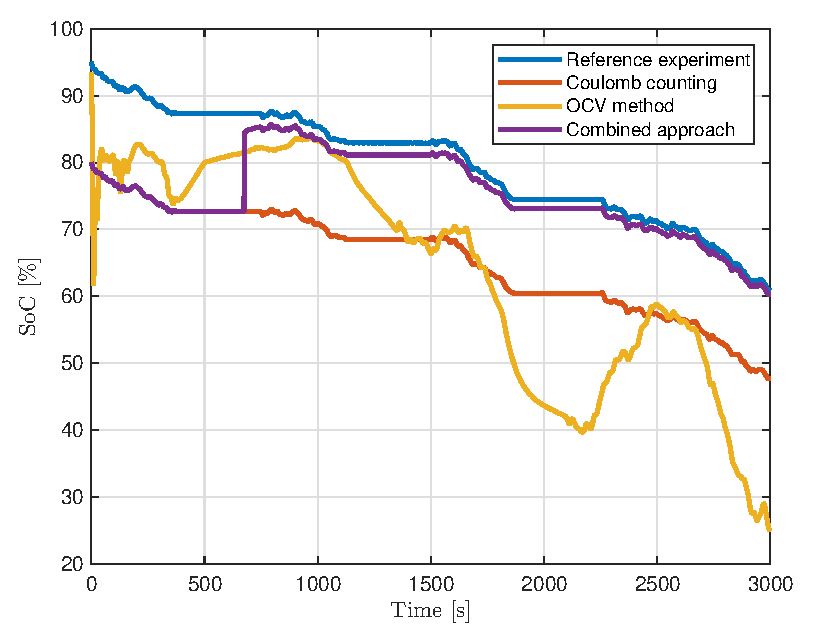
\includegraphics[width=0.5\textwidth]{figures/7/comparison-SOC.eps}
    \caption{Performance comparison of presented estimation algorithms.}
    \label{fig:7-comparison-SOC}
\end{figure}

\section{Discussion}

In this homework, three simple methods of state-of-charge estimation were implemented. The first one -- Coulomb counting -- directly repeatedly evaluates the state equation for $SoC$ using the current measurement $i$. The second method approximates $\OCV$ by filtering terminal voltage measurement $\Ubat$ and subsequently looks the $SoC$ up in a static table. The third method combines both approaches by performing Coulomb counting with occasional resets of the integrator with a value approximated using the $\OCV$.

Key differences between methods can be identified by inspecting Fig. \ref{fig:7-comparison-SOC}, where each method is represented by just one waveform. Each selected waveform does not necessarily minimize the $SoC$ RMSE, but it displays characteristic behavior and disadvantages inherent to the used method. The OCV method, as implemented in Sec. \ref{sec:7-ocv}, leads generally to the "wildest" (and worst) estimate from the customer's point of view. Coulomb counting analyzed in Sec. \ref{sec:7-cc} leads to very accurate estimates of $\Delta SoC$ over short time periods before the integration accumulates significant errors. It is however incapable of yielding absolute $SoC$, since the initial condition for integration is unknown in real applications. Clearly the best performance is achieved by the combined algorithm discussed in Sec. \ref{sec:7-ccr}, because it combines infrequent updates about the absolute $SoC$ from the OCV method with high accuracy relative $\Delta SoC$ calculated by the Coulomb counting.

This conclusion is supported by comparison of root-mean-square errors of estimates; as shown in Fig. \ref{fig:7-validation-SOC}, Coulomb counting is capable of achieving very low RMSE when given exact knowledge of the initial value. The OCV method achieves RMSE of roughly 18 \% or more, as shown in Fig. \ref{fig:7-OCV-SOC}, but it does not depend on the algorithm's initialization. Finally the values in Fig. \ref{fig:7-combination-SOC} show what the combined approach achieves errors as low as 7 \% in spite of very wrong initial estimate of $SoC$. Coulomb counting with reset combines low RMSE of Coulomb counting and robustness to wrong initial conditions characteristic to the OCV method.
